%!TEX root = ../dissertation.tex
%\begin{savequote}[75mm]
%Nulla facilisi. In vel sem. Morbi id urna in diam dignissim feugiat. Proin molestie tortor eu velit. Aliquam erat %volutpat. Nullam ultrices, diam tempus vulputate egestas, eros pede varius leo.
%\qauthor{Quoteauthor Lastname}
%\end{savequote}

\chapter{Ambienti virtualizzati in Android}
\label{chap:virt_env}

La virtualizzazione in \emph{Android} è stata inizialmente ideata per permettere agli sviluppatori di creare applicazioni che oltrepassassero le dimensioni limite imposte. Però la capacità di lanciare molteplici istanze della stessa applicazione senza bisogno di una vera e propria installazione ha portato la virtualizzazione a essere utilizzata per scopi molto diversi. Viene utilizzata per creare degli spazi virtuali, in cui gli utenti possono avviare cloni di applicazioni. Anche molti malware sono stati accusati di utilizzare la virtualizzazione, nascondendo la loro installazione dietro a un'altra un'applicazione ed ereditando i suoi permessi.

La popolarità delle applicazioni che permettono la virtualizzazione è molto rilevante. \emph{Parallel Space} \cite{ParallelSpace}, una delle più famose, è stata scaricata più di 1 milione di volte. Altre applicazioni note che vengono spesso usate sono \emph{Go-Multiple} \cite{GoMultiple} e \emph{Parallel Accounts} \cite{parallelAccounts}. In rete inoltre sono disponibili i sorgenti dei più famosi framework di virtualizzazione, \emph{DroidPlugin} \cite{DroidPlugin}, \emph{VirtualApp} \cite{VirtualApp} e \emph{DynamicAPK} \cite{DynamicAPK} sui quali vengono poi costruite le applicazioni commerciali o i malware.

I rischi principali legati alla virtualizzazione sono la condivisione, da parte di tutte le applicazione ospite, di tutti i permessi dell'applicazione contenitore. Ad esempio un'applicazione ospite potrebbe accedere a dei permessi non dichiarati nel suo \emph{\gls{manifestg}}\glsfirstoccur, ma dichiarati nel \emph{\gls{manifestg}} dell'applicazione contenitore. Inoltre le applicazioni ospite potrebbero anche non essere installate nel dispositivo, ma essere clonate direttamente nell'ambiente di virtualizzazione tramite un \emph{APK}, senza alcuna richiesta. Quindi un'applicazione ospite malevola, installata senza alcuna richiesta, potrebbe accedere ai dati personali, tramite i permessi concessi dall'applicazione contenitore, e inviarli in rete. 

Gli ambienti virtualizzati sono utilizzati anche come strumenti di difesa, come \emph{NJAS} \cite{NJAS} e \emph{Boxify} \cite{Boxify}. Il primo crea un ambiente virtualizzato dove vengono testati potenziali malware evitando che prendano possesso del sistema operativo. Il secondo crea un \emph{\gls{sandboxg}}\glsfirstoccurspace dove le applicazioni possono avviarsi in processi isolati in modo da evitare la condivisione dei permessi.

\newpage

\section{Architettura}

Ci sono diversi modi per implementare un ambiente virtualizzato, ma in linea generale tutti hanno una simile architettura. Le applicazioni contenitore operano a un layer superiore rispetto al framework di \emph{Android} intercettando le chiamate di sistema, attraverso degli \emph{\gls{hookg}}\glsfirstoccur. In generale vengono utilizzati i \emph{dynamic proxy di Java}\cite{DynamicProxy} che rendono semplice l'applicazione di \emph{\gls{hookg}} delle \emph{\gls{apig}} di \emph{Android}. 

Le \emph{API} su cui applicare gli \emph{\gls{hook}} riguardano:
\begin{itemize}
\item l'avvio di un'applicazione tramite \emph{APK} senza installazione;
\item gestione del ciclo di vita di un'applicazione;
\item comunicazione interna tra applicazioni ospite;
\item gestione delle applicazioni ospite.
\end{itemize}

Come si può vedere in Fig.\ref{fig:droidplugin} tutte le applicazioni ospite vengono avviate attraverso\\ un'applicazione contenitore, nella quale vengono applicati gli \emph{\gls{hookg}}, intercettando le chiamate a sistema. Infatti ogni chiamata come \emph{startActivity} o \emph{startService} da un'applicazione ospite passa per l' applicazione contenitore prima di raggiungere il framework di \emph{Android}. Si vede inoltre che tutte le applicazioni avviate all'interno dello stesso ambiente di virtualizzazione condividono lo stesso \emph{\gls{useridg}}\glsfirstoccur, ma ogni applicazione ha il suo \emph{\gls{processidg}}\glsfirstoccur.

\begin{figure} [H]
\centering
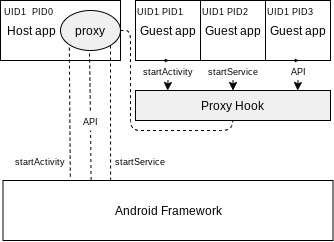
\includegraphics[width=0.6\textwidth]{figures/droidplugin}
\caption[Architettura di DroidPlugin]{Architettura di DroidPlugin
\label{fig:droidplugin}}
\end{figure}

\subsection*{Avvio automatico}

La classe \emph{\gls{classloaderg}} viene utilizzata in \emph{Android} per caricare le classi di un'applicazione da una lista chiamata \emph{DexElement}, che contiene i \emph{\gls{dexfileg}} delle applicazioni. La classe base è \emph{BaseDexClassLoader} che implementa diverse classi come \emph{BootClassLoader}, per caricare le classi di sistema, e \emph{DexClassLoader}, per caricare le classi delle applicazioni.
La classe \emph{DexClassLoader} chiama la funzione \emph{openDexFileNative} per cercare e trovare il path dei \emph{\gls{dexfileg}} interessati. Durante l'installazione di un'applicazione il pacchetto viene estratto, vengono recuperati i \emph{\gls{dexfileg}} e copiati all'interno dell'array \emph{DexElement}.

\emph{DroidPlugin} e \emph{VirtualApp} applicano un \emph{\gls{hookg}} al \emph{ClassLoader}, aggiungendo i \emph{\gls{dexfileg}} delle applicazioni ospite all'interno dell'array \emph{DexElement}. 
In Fig.\ref{fig:BaseDexClassLoader} viene illustrata la classe \emph{BaseDexClassLoader} e in particolare come vengono inseriti i \emph{\gls{dexfileg}} delle applicazioni ospite.

\begin{figure} [H]
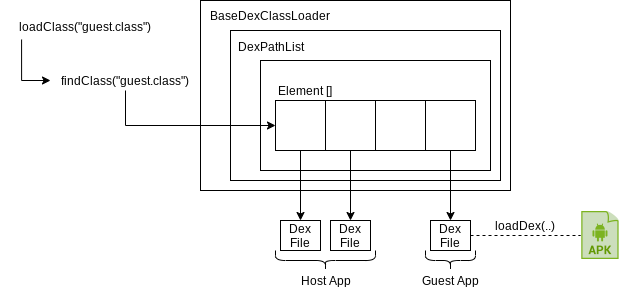
\includegraphics[width=\textwidth]{figures/BaseDexClassLoader}
\caption[Hook della classe ClassLoader]{Hook della classe ClassLoader
\label{fig:BaseDexClassLoader}}
\end{figure}

In questo modo è possibile avviare le applicazioni all'interno di un ambiente virtualizzato, anche senza che siano realmente installate nel dispositivo.

\newpage

\subsection*{Permessi condivisi}

Il gestore dei pacchetti di \emph{Android} genera un \emph{\gls{useridg}} univoco ogni volta che viene installata un'applicazione. Questo comporta che ogni applicazione ospite condividerà lo stesso \emph{\gls{useridg}} dell'applicazione contenitore, ma con differenti \emph{\gls{processidg}}. In questo modo tutti i permessi associati all'applicazione contenitore saranno associati anche alle applicazioni ospite, che condividono lo stesso \emph{\gls{useridg}}. Infatti i malware basati sulla virtualizzazione, per agire, si basano sul concetto dei permessi condivisi.


\subsection*{Componenti predefiniti}

La difficoltà più grande riguarda la gestione di un'applicazione a runtime in un ambiente virtualizzato.
Infatti le applicazioni \emph{Android} non possono creare le \emph{\gls{activityg}}\glsfirstoccurspace da sole, ma hanno bisogno di usare l' \emph{\gls{activitymanagerserviceg}}\glsfirstoccurspace o \emph{AMS}. L'\emph{AMS} viene utilizzato per gestire il ciclo di vita di ogni \emph{\gls{activityg}}. La procedura standard per avviare un'\emph{\gls{activityg}} è chiamare l'\emph{API startActivity}. Dopo la chiamata l'\emph{AMS} si preoccuperà di mettere in pausa l'\emph{\gls{activityg}} corrente e creare quella richiesta. Subito dopo verrà notificato l'\emph{\gls{atg}}\glsfirstoccurspace che caricherà ed eseguirà il codice relativo all'\emph{\gls{activityg}} creata attraverso il metodo \emph{onCreate}.

Il metodo \emph{startActivity} invia un \emph{\gls{intentg}}\glsfirstoccurspace con il contenuto della classe da creare all' \emph{AMS}. Successivamente l'\emph{AMS} invia l'\emph{\gls{intentg}} all'oggetto \emph{\gls{atg}} che chiamerà la funzione di \emph{\gls{callbackg}}\glsfirstoccurspace \emph{handleLaunchActivity}. Questa funzione estrae la classe dell'\emph{\gls{intentg}} per inziare ad eseguire il codice.

Nel caso di un ambiente virtualizzato è necessario applicare degli \emph{\gls{hookg}} per avviare le \emph{\gls{activityg}} o si andrà incontro a un errore visto che le \emph{\gls{activityg}} delle applicazioni ospite non sono dichiarate nel \emph{manifest} dell'applicazione contenitore. \emph{DroidPlugin}, ad esempio, dichiara nel suo \emph{manifest} delle \emph{\gls{activityg}} e dei servizi stub, utilizzati poi per le applicazioni ospite.

A runtime \emph{DroidPlugin} intercetta l'\emph{\gls{intentg}} inviato all'\emph{AMS} dall'\emph{\gls{activityg}} corrente e crea un nuovo \emph{\gls{intentg}} utilizzando lo stub dell'\emph{\gls{activityg}} dichiarata nel manifest di \emph{DroidPlugin}. Inoltre \emph{DroidPlugin} si occupa di consegnare all'oggetto \emph{\gls{atg}} l'\emph{\gls{intentg}} originale.
La stessa procedura è simile per tutti gli altri tipi di componente, come i \emph{\gls{serviceg}}, i \emph{\gls{contentproviderg}}\glsfirstoccurspace o i \emph{\gls{broadcastreceiverg}}\glsfirstoccur.
In Fig. \ref{fig:ams} viene illustrato come vengono avviate le \emph{\gls{activityg}} delle applicazioni ospite.

\begin{figure} [H]
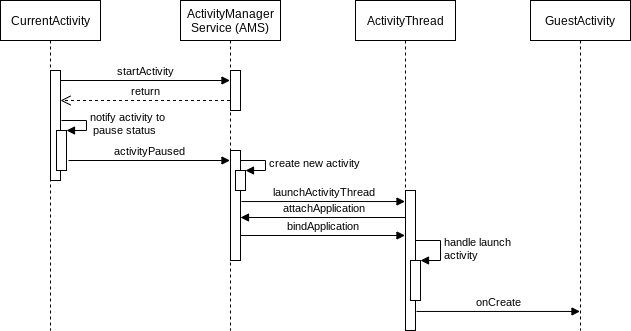
\includegraphics[width=\textwidth]{figures/newactivity}
\caption[Creazione di una nuova activity]{Creazione di una nuova activity
\label{fig:ams}}
\end{figure}


\subsection*{Memoria condivisa}

Di solito a ogni applicazione viene assegnato il suo spazio di memoria privato, garantendo alle altre di non potervi accedere visto l'\emph{\gls{useridg}} diverso.
Negli ambienti virtualizzati l'\emph{\gls{useridg}} viene condiviso da tutte le applicazioni permettendo alle applicazioni ospite di accedere a vicenda ai loro dati privati.
Le directory di installazione solitamente situate in \emph{/data/app/[package]} negli ambienti virtualizzati sono contenute dentro i dati dell'applicazione contenitore in \emph{/data/data/[host]/data/app/[package]}. In questo modo i framework di virtualizzazione riescono ad aggirare la politica di separazione di memoria secondaria dei pacchetti.


\newpage
\section{Attacchi basati sulla virtualizzazione}
\label{sec:attacchi_virt}

Il \emph{\gls{playstoreg}}, contenente più di tre milioni di applicazioni, attira molti sviluppatori a pubblicare la propria applicazione e, sfortunatamente, molti di loro contribuiscono alla pubblicazione di applicazioni malevoli.
Gli attuali meccanismi automatici di identificazione di software malevoli non sono sufficienti a bloccare potenziali applicazioni attaccanti. 

La virtualizzazione viene sfruttata per realizzare malware per i seguenti motivi:
\begin{itemize}
\item \emph{Installazione automatica dei malware dentro le applicazioni contenitore senza bisogno dei permessi di \gls{rootg}\glsfirstoccur}: in questo modo è possibile eseguire aggiornamenti di malware automatici, scaricando e avviando l' \emph{APK} del malware da un server remoto;
\item \emph{Evasione della detection statica, scaricando e avviando le guest app da remoto al loro utilizzo}: è difficile trovare evidenze di codice sospetto in questo modo;
\item \emph{\gls{phishingg} senza ricompilare le applicazioni}: un tempo le applicazioni venivano modificate per effettuare \emph{\gls{phishingg}}, ma al giorno d'oggi sono pochi i casi in cui questa tecnica non sia identificabile. Grazie alla virtualizzazione e alla condivisione di dati tra tutto l'ambiente virtualizzato è possibile creare attacchi virtualizzando due applicazioni ospite, una vittima e l'altra creata appositamente per l'attacco.
\end{itemize}


La popolarità della tecnica della virtualizzazione è confermata dall'alto numero di applicazioni scaricate.
Secondo uno studio del \emph{Tencent security lab}\cite{TencentSecLab} solo l' 8.86\% delle applicazioni che utilizzano \emph{VirtualApp} non hanno scopi maligni.
Grazie alla condivisione dello stesso \emph{\gls{useridg}} da parte di tutte le applicazioni ospite e dell'applicazione contenitore i permessi vengono ereditati a tutte le applicazioni e la memoria secondaria è condivisa.
Le tipologie di attacchi che sfruttano la virtualizzazione sono generalmente due:
\begin{itemize}
    \item \emph{duplicazione di applicazioni per permettere all'utente di avere più account simultaneamente}: gli attaccanti applicano degli \emph{\gls{hookg}} ai campi di input \emph{EditText} all'applicazione duplicata e inviano le informazioni inserite dall'utente a un server esterno;
    \item \emph{aggiornamento di un'applicazione già esistente nel dispositivo}: gli attaccanti diffondono un add-on di un'applicazione con lo scopo di aggiungere funzionalità. Ma in realtà viene creato anche un ambiente virtualizzato al fine di accedere ai dati sensibili tramite i permessi.
\end{itemize}

\subsection*{Màscara}

Un esempio di malware che sfrutta la virtualizzazione è \emph{Màscara}.
Il nome \emph{Màscara}, maschera in veneziano, si addice perfettamente alla tipologia di malware, infatti \emph{Màscara} crea un ambiente virtualizzato sopra un'applicazione vittima, come una maschera.
Attraverso questo malware sarà dimostrata la pericolosità degli ambienti virtualizzati e la facilità nel superare le tecniche di identificazione attualmente esistenti.

La particolarità di questo malware è la compatibilità con qualsiasi applicazione. Tramite il framework \emph{Màscarer} è possibile infatti generare, a partire da un \emph{APK} vittima, un \emph{APK} add-on da installare nel dispositivo (\emph{Màscara}), e un \emph{APK} malevolo, che verrà scaricato e installato dall'applicazione add-on a runtime.

\emph{Màscara} è stato sviluppato sopra \emph{DroidPlugin} che permette di realizzare un attacco più pericoloso rispetto agli altri framework di virtualizzazione come \emph{VirtualApp} oppure \emph{DynamicAPK}. 
Tramite \emph{DroidPlugin} è possibile infatti avviare una o più applicazioni contemporaneamente e avviare applicazioni non installate nel dispositivo.
In Fig.\ref{fig:persona_arch} è mostrata l' architettura di \emph{Màscara}.


\begin{figure} [H]
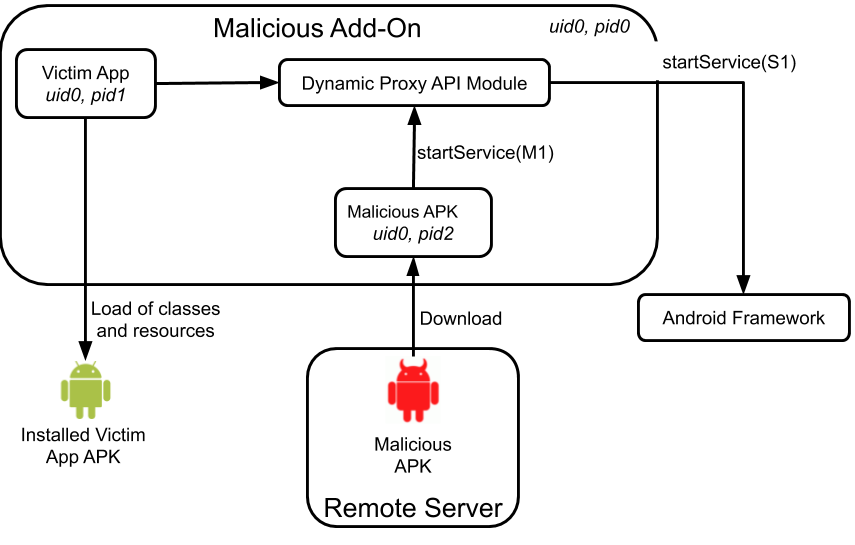
\includegraphics[width=\textwidth]{figures/PersonaArchitecture}
\caption[Architettura dell'add-on di Màscara]{Architettura dell'add-on di Màscara
\label{fig:persona_arch}}
\end{figure}
\newpage

L'add-on contiene \emph{DroidPlugin} che viene rappresentato come un contenitore. Al suo interno viene avviata l'applicazione vittima e l'\emph{APK} malevolo. Le due applicazioni ospite condividono lo stesso \emph{\gls{useridg}}.

Lo scenario di un attacco è rappresentato in Fig. \ref{fig:scen_attacc}:
\begin{enumerate}
\item L'attaccante genera l'add-on malevolo, tramite \emph{Màscarer}, di un'applicazione a sua scelta. Dopo aver realizzato l'add-on pubblica l'applicazione nel \emph{\gls{playstoreg}}, la quale analisi statica non riesce rilevare la presenza di codice malevolo dato che viene scaricato a runtime;

\item L'utente inconsapevole scarica l'applicazione add-on dal \emph{\gls{playstoreg}} con lo scopo di aggiungere funzionalità all'applicazione vittima. Risulta essere una pratica molto comune la realizzazione di applicazioni add-on per altre applicazioni, anche per scopi benigni;

\item Una volta che l'utente installa l'add-on nel dispositivo e lo avvia, viene creato un collegamento nel \emph{\gls{launcherg}}\glsfirstoccurspace a \emph{DroidPlugin} con la stessa icona dell'applicazione originale;

\item L'applicazione vittima viene avviata all'interno del contenitore in un ambiente virtualizzato, se si avvia l'applicazione tramite il nuovo collegamento;

\item L'\emph{APK} malevolo viene successivamente scaricato da un server esterno ed installato all'interno del contenitore e avviato. L'applicazione malevola appena scaricata a questo punto eredita tutti i permessi dell'applicazione vittima e può iniziare a inviare dati sensibili a un server esterno. \emph{Màscara} cercherà infine di inviare al server delle foto scattate al momento senza alcun avviso, i contatti, gli sms, dimostrando i problemi di sicurezza degli ambienti virtualizzati.
\end{enumerate}
\begin{figure}
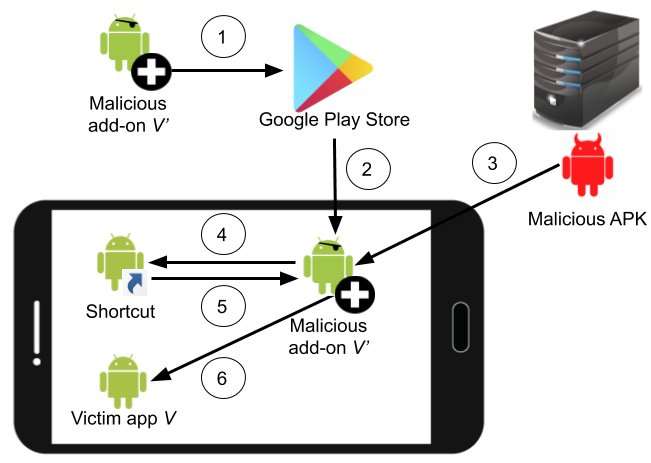
\includegraphics[width=\textwidth]{figures/PersonaAttackScenario}
\caption[Scenario dell'attacco Màscara]{Scenario dell'attacco
\label{fig:scen_attacc}}
\end{figure}

